\doublespacing % Do not change - required

\chapter{Background}
\label{ch:background}

%%%%%%%%%%%%%%%%%%%%%%%%%%%%%%%%%%%%%%%
% IMPORTANT
\begin{spacing}{1} %THESE FOUR
\minitoc % LINES MUST APPEAR IN
\end{spacing} % EVERY
\thesisspacing % CHAPTER
% COPY THEM IN ANY NEW CHAPTER
%%%%%%%%%%%%%%%%%%%%%%%%%%%%%%%%%%%%%%%

% Transplanted from the Interim Report background chapter. Per the FYP guide,
% reusing Interim material here is allowed and encouraged.

\section{Applications of Near-Infrared Imagery}
\label{sec:nir_applications}

Near-infrared (NIR) imagery is used across scientific, industrial and security applications because it captures information beyond the visible spectrum. Biometrics is a prominent example. NIR is used for palm, face and vein recognition~\cite{s17061297}: it penetrates deeper into skin than visible light and exposes subsurface features such as blood vessels, which makes it more robust to skin tone, makeup and ambient lighting. It also suppresses the shadows and highlights of uneven illumination, helping face recognition in unconstrained settings. Palm- and finger-vein systems rely almost entirely on NIR, since haemoglobin absorbs it and produces high-contrast vascular patterns that are invisible in RGB (\autoref{fig:hand_nir})~\cite{miura2004feature,li2007illumination,Bashkatov_2005}.

\begin{figure}[!htbp]
    \centering
    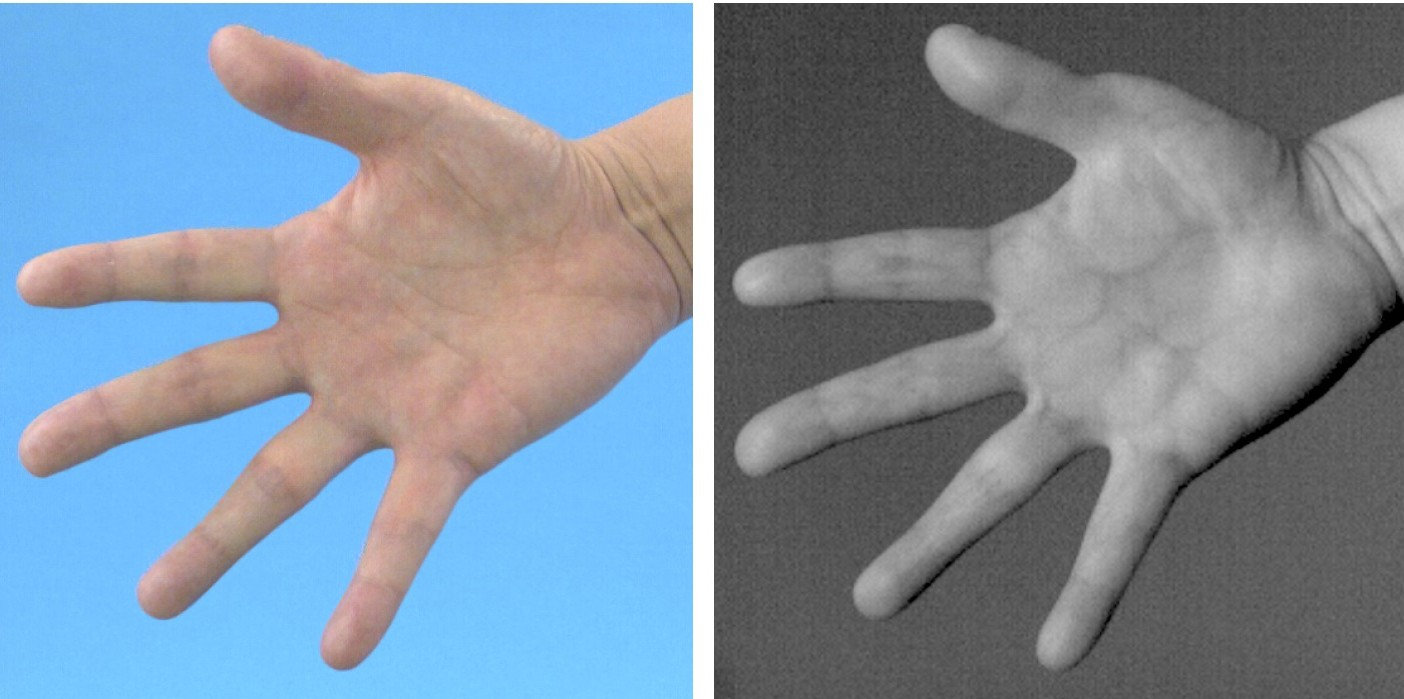
\includegraphics[width=0.8\textwidth]{imgs/nir-hand.jpg}
    \caption{Left image is RGB, right image is NIR. Figure reproduced from~\cite{Monno2019RGBNIR}.}
    \label{fig:hand_nir}
\end{figure}

Remote sensing and environmental monitoring is another major use. Vegetation reflects NIR strongly because of its spongy mesophyll structure, which supports robust assessment of plant health, biomass, crop yield and drought~\cite{tucker1979red}. Unlike RGB, which is sensitive to illumination and surface colour, NIR gives a more stable measure of vegetation health.

NIR is also common in surveillance, night vision and autonomous driving. With active infrared illumination it images in low light and at night, where RGB cameras fail, and its longer wavelengths scatter less, which helps perception in fog or haze~\cite{he2011single}. In industrial inspection it supports material sorting, quality control and defect detection, since materials differ in NIR reflectance.

\section{Spectral Characteristics and Physics of NIR}
\label{sec:nir_physics}

NIR sits just beyond visible red, but what makes it useful is how it interacts with matter. Visible-light imaging mostly sees surface reflectance from pigments and dyes. NIR reflectance instead depends on molecular vibrations, water content and a material's internal structure~\cite{curran1989remote}. Because NIR also scatters and is absorbed less in organic matter, it penetrates further into skin, leaves and other semi-translucent subjects, picking up subsurface detail that visible light never reaches.

Materials that look distinct in RGB can look identical in NIR, and the reverse also happens. Healthy vegetation is green in RGB, because chlorophyll absorbs red and blue, but very bright in NIR, since chlorophyll does not absorb NIR (\autoref{fig:leaf_nir}). Water absorbs NIR strongly and appears dark, which makes NIR effective for water-body delineation and moisture analysis~\cite{gao1996ndwi}.

\begin{figure}[!htbp]
    \centering
    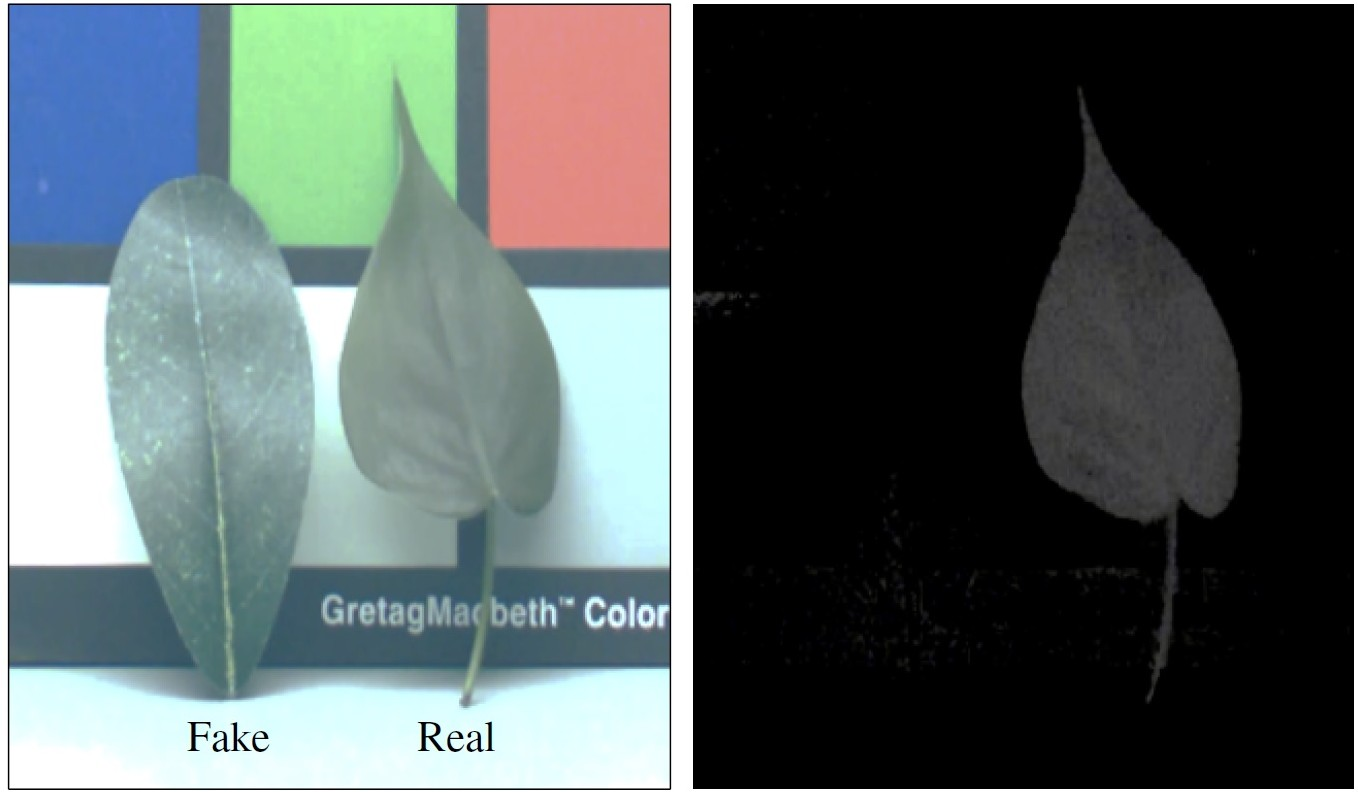
\includegraphics[width=0.8\textwidth]{imgs/leaf-nir.jpg}
    \caption{Left image is RGB, right image is NIR. Figure reproduced from~\cite{Monno2019RGBNIR}.}
    \label{fig:leaf_nir}
\end{figure}

\section{Visual and Textural Differences: NIR vs.\ RGB}
\label{sec:nir_rgb_differences}

The two bands diverge most in texture. In RGB, texture comes from colour gradients, shading and surface pigmentation. In NIR it comes from material composition, moisture and internal structure, which pushes edges, contrast and spatial-frequency content away from anything an RGB-trained model expects~\cite{salamati2010material,salamati2014incorporating}.

For example, skin looks uniform in RGB, its texture set by pores, wrinkles and pigmentation, but smoother in NIR, where subsurface veins become prominent (\autoref{fig:hand_nir}). Facial hair, prominent in RGB, is darker and less distinct in NIR, and fabrics with different RGB colours can look identical in NIR when the material is the same.

NIR is also less affected by shadows and specular highlights, giving smoother gradients and different edge responses. Convolutional filters and descriptors trained on RGB therefore behave differently on NIR. This mismatch in texture, contrast and spatial statistics is the core difficulty in cross-spectral understanding that NIR-to-RGB translation sets out to address.

\section{Impact on Machine Learning Performance}
\label{sec:nir_ml_impact}

These spectral and textural differences degrade machine-learning models trained only on RGB. Deep networks implicitly learn RGB statistics such as colour distributions, channel correlations and texture~\cite{krizhevsky2012imagenet}, and on NIR input those learned features often fail to fire because the input assumptions are violated. \autoref{fig:yolo_nir_rgb} compares the Ultralytics YOLOv8 Nano detector~\cite{jocher2023yolov8} on NIR and RGB.

\begin{figure}[!htbp]
    \centering
    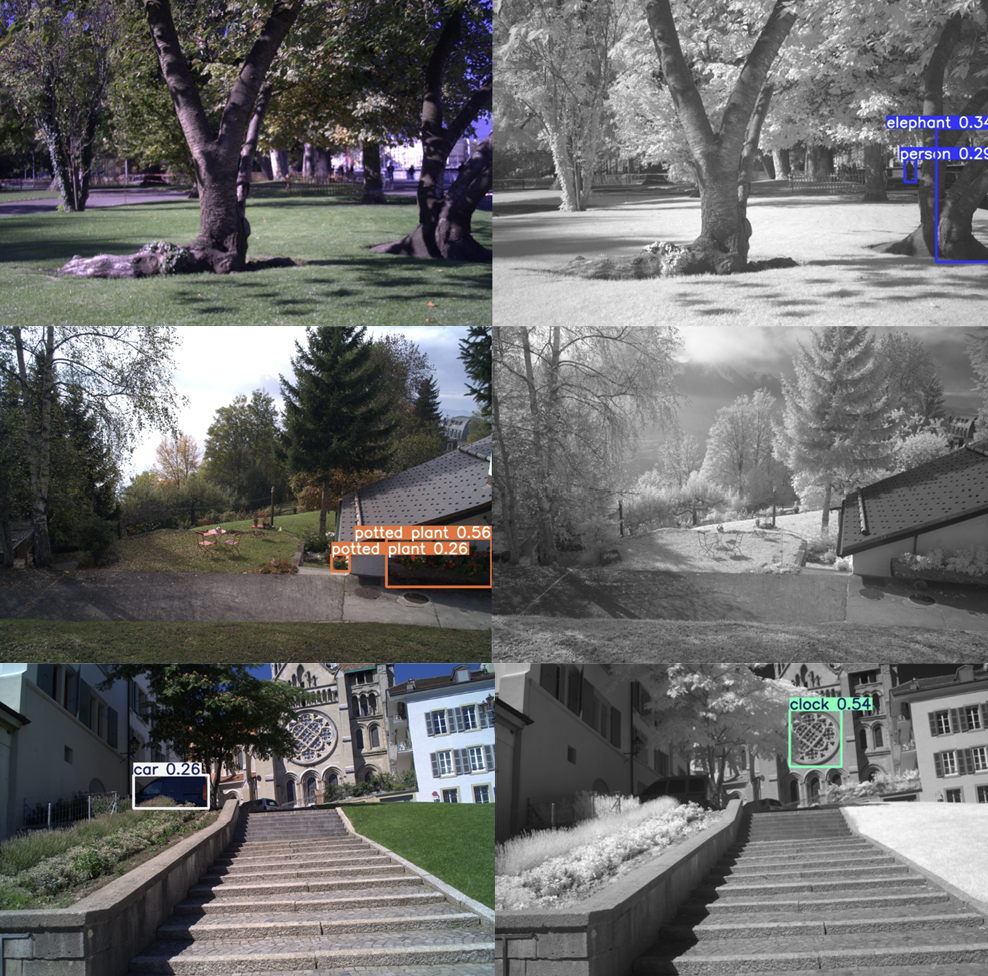
\includegraphics[width=0.8\textwidth]{imgs/poor.png}
    \caption{Ultralytics YOLOv8 Nano detector run on an RGB image (left) and the matching NIR image (right). NIR/RGB images from the EPFL RGB-NIR Scene Dataset~\cite{epfl_rgbnir_dataset}.}
    \label{fig:yolo_nir_rgb}
\end{figure}

Segmentation, detection and face-recognition models lean on colour and visible texture to separate classes. NIR lacks colour and has different intensity statistics, so early filters tuned for RGB edges and colour give weak or misleading activations~\cite{peng2018rgbnir,salamati2014incorporating}, and the models generalise poorly even when the semantic content is unchanged. \autoref{fig:nir_rgb_comparison} shows a segmentation model failing on a simple NIR case.

\begin{figure}[!htbp]
    \centering
    \begin{minipage}{0.39\textwidth}
        \centering
        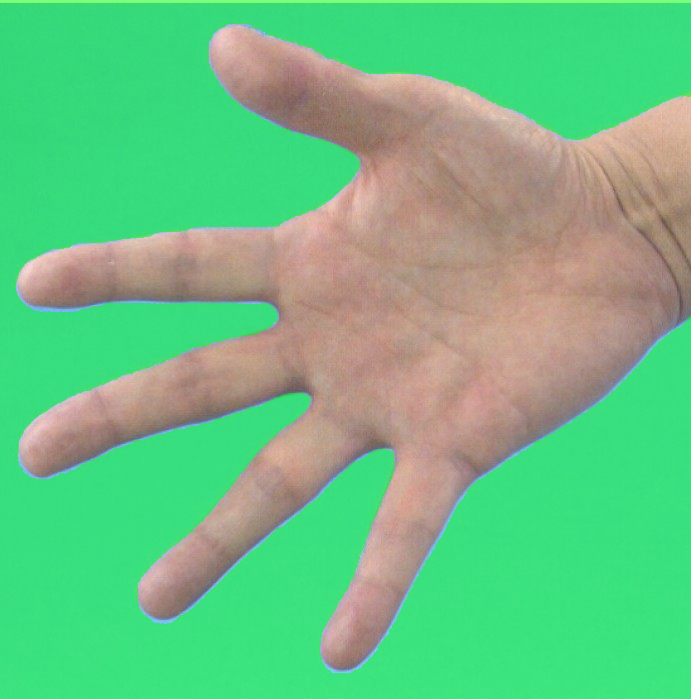
\includegraphics[width=\linewidth]{imgs/nir-hand2_mediapipe_overlay.png}
        \subcap{(a) RGB image}
    \end{minipage}
    \hspace{0.002\textwidth}
    \begin{minipage}{0.39\textwidth}
        \centering
        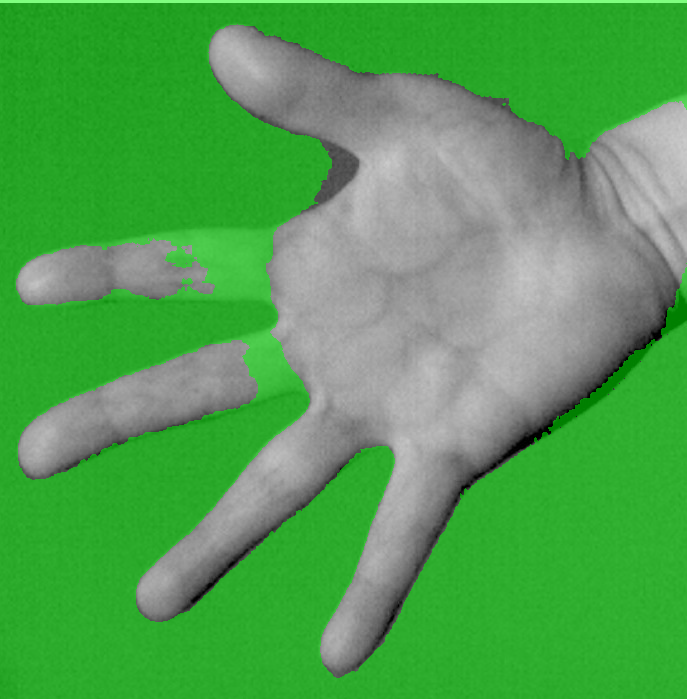
\includegraphics[width=\linewidth]{imgs/nir-hand1_mediapipe_overlay.png}
        \subcap{(b) NIR image}
    \end{minipage}
    \caption{Background (green overlay) segmentation from the MediaPipe Selfie Segmentation model~\cite{lugaresi2019mediapipe}. The same model fails to find a foreground subject on the NIR input.}
    \label{fig:nir_rgb_comparison}
\end{figure}

Although the NIR camera records a three-channel image, all three channels sample the same band beyond the 850\,nm filter, so they are highly correlated and carry no colour information: the input is spectrally single-band even though it is stored as three channels. This removes the cross-channel structure that RGB models rely on for robustness. Translating NIR to RGB is therefore a practical adaptation strategy: it produces RGB-like images that better match the feature space of pretrained RGB models~\cite{isola2017image}.

While the examples above use single detectors, the degradation is systematic across architectures rather than an artefact of one model. To confirm this on the data collected for this project (Chapter~\ref{ch:implementation}), a panel of nine modern semantic-segmentation transformers was run on paired NIR and RGB frames. The panel covers SegFormer~\cite{xie2021segformer}, BEiT~\cite{bao2022beit} and Mask2Former~\cite{cheng2022mask2former} variants trained on the ADE20K~\cite{zhou2017ade20k} and Cityscapes~\cite{cordts2016cityscapes} benchmarks, and for each model the agreement between its NIR and RGB segmentations was measured per object category. The loss of agreement is substantial but non-uniform. Vegetation and person regions, whose NIR appearance departs most from the visible band, degrade far more than road or building surfaces, and the smaller, more deployable models degrade more than the larger ones. This last point is particularly important in an edge setting, since the efficient models most likely to be deployed are also the most fragile on NIR input. This motivates placing a lightweight NIR$\rightarrow$RGB translator ahead of them. The downstream evaluation of Chapter~\ref{ch:results} measures how much of that agreement the translator developed here restores for the panel's most deployable architecture, SegFormer-B0, on both its ADE20K and Cityscapes variants (Section~\ref{sec:res_seg}).

Figures~\ref{fig:seg_fail_mask2former} and \ref{fig:seg_fail_beit} make these failure modes concrete for two of the panel's architectures. In each, the top row shows the RGB and raw-NIR inputs and the bottom row the corresponding segmentations. The overlay colours are green for vegetation, yellow for buildings, red for people and blue for road, and the per-category Dice agreement with the RGB segmentation is printed on each example. They show that the collapse is selective. Classes whose NIR appearance departs most from the visible band fail, while structurally similar surfaces such as road are often preserved.

\begin{figure}[!htbp]
    \centering
    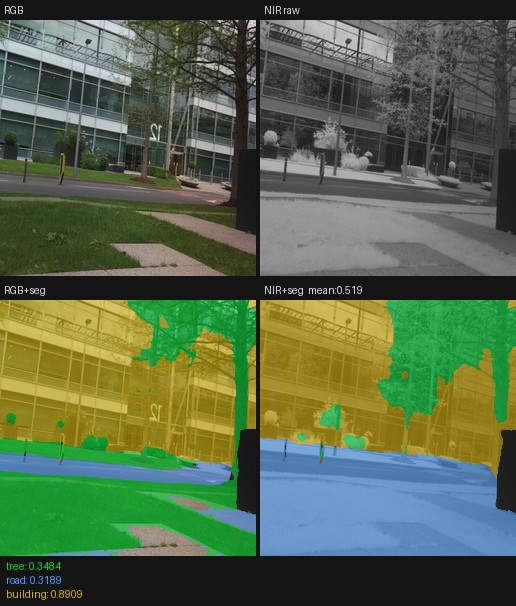
\includegraphics[width=0.78\textwidth]{imgs/mask2former-fail.jpg}
    \caption{Mask2Former (ADE20K) Overlay key: green = vegetation, yellow = building, red = person, blue = road. The building is largely recovered on NIR (Dice 0.89), but the bright NIR foliage and pavement are misread: vegetation collapses to 0.35 and the path is misclassified as road (0.32).}
    \label{fig:seg_fail_mask2former}
\end{figure}



\begin{figure}[!htbp]
    \centering
    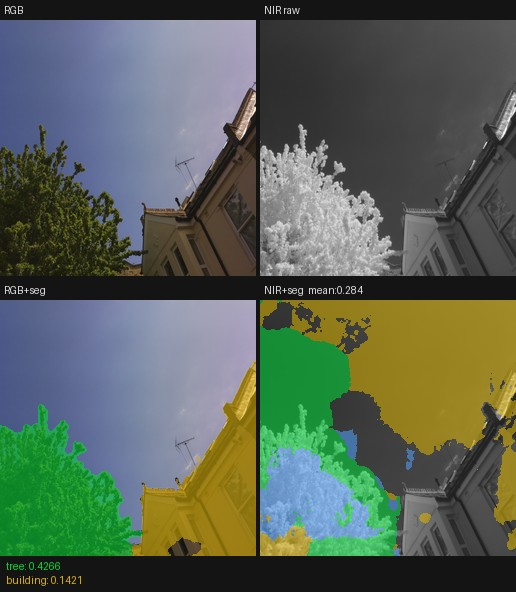
\includegraphics[width=0.78\textwidth]{imgs/beit-fail.jpg}
    \caption{BEiT (ADE20K) on a building and tree scene against sky (mean Dice 0.28)}
    \label{fig:seg_fail_beit}
\end{figure}

\section{Image-to-Image Conversion}
\label{sec:i2i_overview}

Image-to-image conversion learns a mapping between two visual representations of the same content. Modern methods are data-driven, learning non-linear mappings from paired or unpaired data rather than using hand-crafted transforms. For NIR-to-RGB the goal is to turn near-infrared images into plausible RGB while preserving semantic and structural content. This is hard because the NIR input has no colour, so many RGB appearances fit the same NIR observation~\cite{gonzalez2002digital}.

The same problem can be framed as domain adaptation: the translator maps a source distribution $P_{\text{NIR}}$ onto a target distribution $P_{\text{RGB}}$, so that models trained on $P_{\text{RGB}}$ continue to work on inputs originally drawn from $P_{\text{NIR}}$ without retraining~\cite{bendavid2010theory}. This connects NIR-to-RGB translation to the wider literature on covariate shift and feature alignment, and to image-translation-based adaptation methods such as CyCADA~\cite{hoffman2018cycada}, which use a learned image translator as the adaptation mechanism rather than retraining the downstream model. The approach taken in this project follows that pattern: instead of fine-tuning the frozen RGB-pretrained models for NIR input, the input distribution is mapped toward the one those models were trained on.

\subsection{Pre-Deep Learning Approaches}
\label{sec:i2i_classical}

Before deep learning, cross-spectral conversion relied on classical signal processing: linear or piecewise-linear intensity mappings, histogram equalisation and specification to align global statistics, and patch-based methods that matched source patches against a target-domain dictionary~\cite{efros1999texture}. These techniques are computationally cheap, but they either ignore spatial context entirely or depend on handcrafted features that break down under large scene variation. They lack the capacity to model the non-linear, context-sensitive NIR-to-RGB relationship, which motivated the shift to learning-based methods.

\subsection{Deep Learning for Image-to-Image Conversion}
\label{sec:i2i_dl}

Deep learning enabled end-to-end conversion with convolutional neural networks (CNNs). Early models used encoder--decoder architectures: the encoder compresses the input to a latent representation and the decoder reconstructs the target-domain image. These learn spatially varying transforms and capture semantic context, which suits cross-spectral conversion~\cite{dong2015image}.

Fully convolutional networks with skip connections, such as U-Net~\cite{ronneberger2015unet}, were a key step. Skip connections pass low-level spatial detail from early layers straight to later ones, preserving fine detail and sharp edges. That matters for NIR-to-RGB, where structure must be kept while colour is synthesised.

Pixel losses (L1 or L2) enforce fidelity to the ground-truth RGB but blur outputs, since they average over plausible solutions. Perceptual losses address this limitation by comparing high-level features from pretrained networks rather than raw pixels, giving sharper, more semantically meaningful results~\cite{johnson2016perceptual}.

\subsection{Generative Adversarial Networks}
\label{sec:i2i_gan}

A generative adversarial network (GAN) trains a generator against a discriminator so the output matches the target domain's statistics, not just its mean pixel values~\cite{goodfellow2014generative}. The paired variant, the conditional GAN, adds a reconstruction term that ties the output back to the input~\cite{isola2017image}. For aligned NIR/RGB captures this provides a natural baseline: the reconstruction term constrains structure while the adversarial term encourages target-domain appearance.

Pix2pix is the standard cGAN for paired translation: a U-Net generator for spatial detail, a PatchGAN discriminator for local realism, and an L1 reconstruction term~\cite{isola2017image}. Since its introduction it has become the de facto baseline for paired image-to-image translation, and the dominant methods that followed are direct descendants of it, including the high-resolution Pix2pixHD~\cite{wang2018pix2pixhd}, semantic-conditioned SPADE~\cite{park2019spade}, and, in the cross-spectral setting closest to this work, Pix2Next~\cite{pix2next2024}. It is also applied directly to cross-spectral RGB/NIR translation, for example mapping RGB to NIR for fire detection~\cite{akagic2023rgbnir}. It was used as the baseline here because it is straightforward to train and export, and because it is the established formulation any more complex method should be expected to improve on.

\subsection{Limitations of pix2pix for NIR-to-RGB}
\label{sec:pix2pix_limitations}

Three limitations of pix2pix are particularly important in the cross-spectral setting. First, it assumes well-aligned pairs. Even a few pixels of NIR/RGB misregistration can be learned as colour ``halos'' or edge ghosting, while precise pairs are difficult to collect (Section~\ref{sec:datasets}). Second, the mapping is one-to-many because colour is not directly present in the NIR input. An L1-trained deterministic generator can therefore converge toward dataset-average colours and mis-colour materials that share similar NIR responses. Third, the PatchGAN objective rewards local realism, which can produce globally inconsistent texture, subtle tiling or over-sharpening that appears acceptable in small crops but less coherent in full frames. These limitations do not prevent pix2pix from serving as a baseline, but they identify the main areas in which a better translator must improve.

\subsection{Pix2pixHD: high-resolution conditional GANs}
\label{sec:pix2pixhd}

Pix2pixHD scales pix2pix to high resolution~\cite{wang2018pix2pixhd}. Two of its ideas remain especially relevant: a coarse-to-fine generator that establishes global layout before adding fine detail, and multi-scale discriminators that evaluate coarse structure and local texture separately rather than at one fixed patch size. It also adds a feature-matching loss on discriminator activations, which stabilises training and discourages the generator from satisfying the PatchGAN through high-frequency artefacts at the expense of semantic consistency. This feature-matching idea is important for the present project, where matching intermediate representations becomes a way to preserve structure while adapting appearance (Chapter~\ref{ch:design}).

\subsection{Pix2Next: Vision foundation models for RGB$\rightarrow$NIR translation}
\label{sec:pix2next}

Pix2Next is the closest prior work to this project, even though it runs in the opposite direction, RGB$\rightarrow$NIR~\cite{pix2next2024}. It incorporates a frozen pretrained vision model into a Pix2pixHD-style backbone and injects those global features into the generator through cross-attention, so the colour synthesised at a pixel can draw on the whole scene rather than a local patch. Training adds SSIM and feature-matching terms to the adversarial loss to preserve structure.

Two aspects of Pix2Next shaped the approach taken here. First, global features from a large pretrained model provide a practical way to maintain scene-level coherence when paired data are limited. Second, Pix2Next evaluates not only image similarity but also whether the generated output improves a downstream detector. This project adopts the same principle for the reverse NIR$\rightarrow$RGB direction: evaluation is centred on downstream model behaviour rather than image-quality scores alone (Chapter~\ref{ch:design}). Across this line of work, from the perceptual loss~\cite{johnson2016perceptual} through Pix2pixHD's feature matching to Pix2Next's pretrained conditioning and SPADE-style semantic conditioning~\cite{park2019spade}, the common thread is to keep a pretrained network's intermediate activations similar before and after translation, which is the idea the design of this project builds on (Chapter~\ref{ch:design}).

\subsection{Diffusion and Bridge Models for Image-to-Image Conversion}
\label{sec:i2i_diffusion}

Diffusion models generate by iterative denoising: noise is added gradually and the reverse process learns to remove it~\cite{ho2020denoising}. Conditioned on an input such as NIR, they capture the one-to-many ambiguity of colour and produce high-quality, diverse samples, and they train more stably than GANs~\cite{saharia2022image}. In principle, this is well suited to NIR$\rightarrow$RGB, where one NIR frame admits several plausible colourings. Bridge models, including Schr\"odinger bridges, extend the same idea by learning a stochastic transport between two distributions under fixed endpoints, and recent methods are competitive on translation tasks~\cite{leonard2013survey,debortoli2021neural}. Both families, however, share two properties that conflict with this project's deployment target: inference is iterative, requiring many network passes per image, and it is stochastic. Why these properties rule them out here is set out in Section~\ref{sec:why_not_diffusion}.

\subsection{Efficient Restoration Networks for Edge Translation}
\label{sec:i2i_nafnet}

The generative families above (conditional GANs, diffusion and bridge models) prioritise sample realism and the ability to represent one-to-many ambiguity, but they incur either adversarial instability or many denoising steps per image. This cost is difficult to reconcile with a translator that must run deterministically within a small per-frame budget on an edge device. A separate line of work, image restoration, offers an alternative: efficient feed-forward CNNs that map a degraded image to a clean one in a single pass. NAFNet (Nonlinear Activation-Free Network)~\cite{chen2022nafnet} is a prominent example. It reaches state-of-the-art results on denoising and deblurring while stripping the architecture back to a minimal operator set, replacing every nonlinear activation with a multiplicative ``SimpleGate''. That minimal, predictable operator set makes it attractive for constrained hardware, since it exports cleanly to embedded inference runtimes and behaves well under low-bit quantisation.

Restoration networks are usually designed for same-modality problems, where input and output show the same scene under the same imaging conditions (for example noisy$\rightarrow$clean). In that setting the network primarily removes a degradation rather than inferring missing spectral information. NIR$\rightarrow$RGB is harder: colour absent from the input must be inferred from material, texture and scene context. For this reason, using a restoration backbone for cross-spectral translation is a non-standard choice. Prior NIR$\rightarrow$RGB work has more often used generative architectures such as cycle-consistent or conditional GANs, and more recently diffusion models (Sections~\ref{sec:i2i_gan}--\ref{sec:i2i_diffusion}). The literature reviewed for this report did not identify previous use of NAFNet for NIR$\rightarrow$RGB translation. Its strong feed-forward capacity and quantisation-friendly, activation-free design make it a strong candidate for an edge-deployable translator.

\subsection{Availability of Paired RGB--NIR Datasets (and Practical Limitations)}
\label{sec:datasets}

Publicly available RGB--NIR paired datasets exist, but they are relatively small and often are not perfectly paired. A commonly used example is the RGB--NIR Scene Dataset released with Brown and S\"usstrunk's multispectral SIFT work~\cite{brown2011multispectral,epfl_rgbnir_dataset}. It contains aligned RGB and NIR images across several outdoor scene categories, but the RGB and NIR frames are captured using separate exposures with different filters (visible vs.\ NIR, with a cutoff around 750\,nm) and then registered using SIFT~+~RANSAC~\cite{epfl_rgbnir_dataset}. While this produces useful approximate alignment, any motion between NIR and RGB captures (cars, pedestrians, foliage, water) leads to non-matching content. \autoref{fig:epfl_rgbnir_dataset} shows an example of this. Content differences of this kind make such data unsuitable as supervised training pairs for NIR$\rightarrow$RGB translation, because the network would be penalised for failing to reproduce people and objects that are not in the same place in the target frame. This limitation directly motivates the bespoke capture rig built for this project, which images both bands through a shared aperture so that every pair is simultaneous and related by a single depth-independent homography (Chapter~\ref{ch:implementation}).

\begin{figure}[!htbp]
    \centering
    \begin{minipage}[b]{0.42\textwidth}
        \centering
        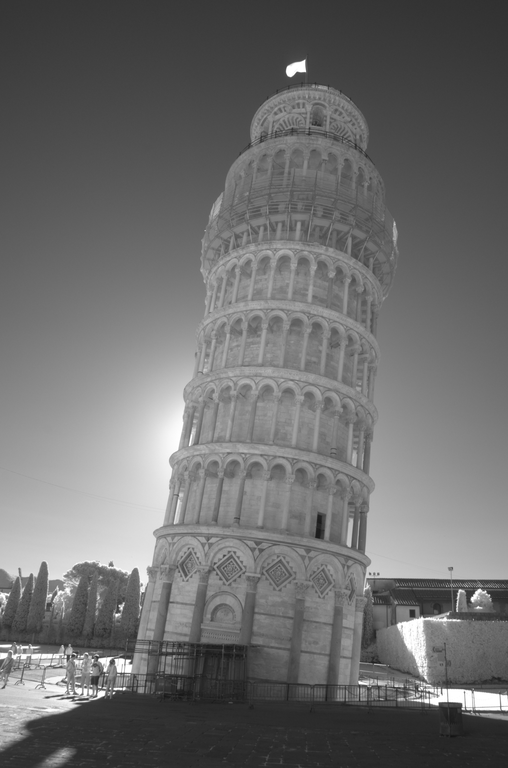
\includegraphics[width=\linewidth]{imgs/0001_nir.png}
        \subcap{(a) NIR image}
    \end{minipage}\hfill
    \begin{minipage}[b]{0.42\textwidth}
        \centering
        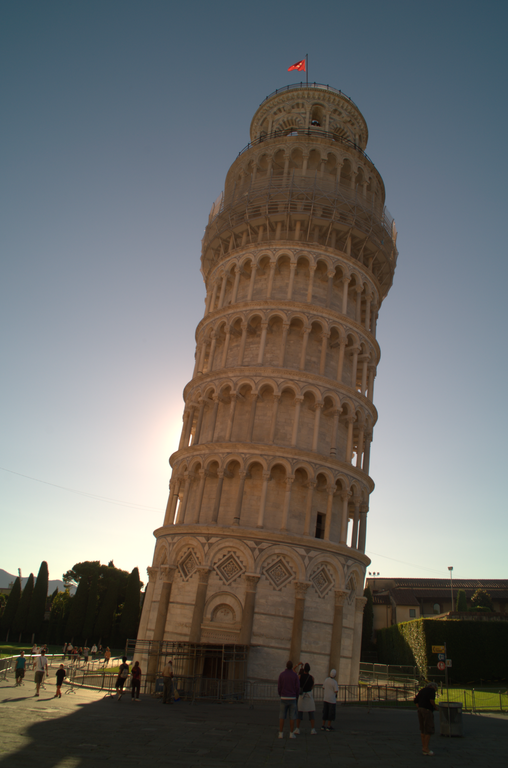
\includegraphics[width=\linewidth]{imgs/0001_rgb.png}
        \subcap{(b) RGB image}
    \end{minipage}
    \caption{An imperfectly paired sample from the EPFL RGB--NIR Scene Dataset~\cite{epfl_rgbnir_dataset,brown2011multispectral}. The tower aligns across bands, but the pedestrians in the foreground have moved between the two exposures. This is a content mismatch that post-hoc registration cannot correct.}
    \label{fig:epfl_rgbnir_dataset}
\end{figure}

\section{Model Compression for Edge Deployment}
\label{sec:model_compression}

A translator that reaches high image quality is usually too large to run inside a per-frame budget on an edge device. The gap between a strong model and a deployable one is normally closed with two complementary techniques: knowledge distillation, which trains a small network to behave like a large one, and quantisation, which stores and computes that network at lower numerical precision. Both are used in this project, so the underlying ideas are summarised here before the design and implementation chapters apply them.

\subsection{Knowledge Distillation}
\label{sec:kd}

Knowledge distillation trains a compact student network to reproduce the behaviour of a larger teacher rather than learning the task from labels alone~\cite{hinton2015distilling}. The original formulation matches the teacher's softened output distribution, on the argument that the teacher's full response carries more information than a hard target. Later work showed that the student can also be supervised on the teacher's intermediate activations, so that it imitates how the teacher represents an input and not only what it predicts~\cite{romero2015fitnets}.

For image translation the same idea applies at the level of pixels and features. The student is trained to reproduce the teacher's output image, optionally with a small anchor to the ground truth, and can additionally be asked to match feature representations extracted from frozen networks. This is the route taken for the edge model in this project, where a width-16 student is distilled from the width-64 teacher (Chapter~\ref{ch:implementation}).

\subsection{Quantisation}
\label{sec:quantisation}

Quantisation represents weights and activations with lower-precision integers, typically 8-bit (INT8) instead of 32-bit floating point. This shrinks the model and, more importantly on a CPU, lets inference use faster integer kernels~\cite{jacob2018quantization,gholami2021survey}. The two common regimes differ in when quantisation is introduced. Post-training quantisation (PTQ) converts an already-trained model, calibrating the integer ranges from a small set of representative images and requiring no further training. Quantisation-aware training (QAT) instead simulates the rounding during training so the network can adapt to it, which usually recovers more accuracy~\cite{jacob2018quantization}.

This work uses PTQ. The activation-free design of the chosen backbone (Section~\ref{sec:i2i_nafnet}) provides a compact operator set for mixed-INT8 export, although unsupported LayerNorm and PixelShuffle-adjacent operations remain in FP32. The implementation compares static and Q/DQ export paths, and Chapter~\ref{ch:results} reports off-device numerical equivalence and quality retention. On-device latency and memory are measured on the Raspberry~Pi~5 in Section~\ref{sec:res_edge}.
